% latex uft-8
\documentclass[uplatex,a4paper,11pt,oneside,openany]{jsarticle}
%
\usepackage[T1]{fontenc}
\usepackage[dvipdfmx]{graphicx}
\usepackage[dvipdfmx]{color}
\usepackage{amsmath,amssymb}
\usepackage{enumerate}
\usepackage{bm}
\usepackage{graphicx}
\usepackage{ascmac}
\usepackage{setspace}
\usepackage{here}
\usepackage{url}
\usepackage{ulem}
\usepackage{colortbl}
\usepackage{comment}
\usepackage{setspace}
\usepackage{multicol}
\usepackage{multicolpar}
\usepackage{listings,jlisting} %日本語のコメントアウトをする場合jlistingが必要
%ここからソースコードの表示に関する設定
\lstset{
	%プログラム言語(複数の言語に対応,C,C++も可)
	language = Python,
	%背景色と透過度
	backgroundcolor = {\color[gray]{.95}},
	%枠外に行った時の自動改行
	breaklines = true,
	%自動改行後のインデント量(デフォルトでは20[pt])
	breakindent = 10pt,
	%標準の書体
	%basicstyle = \ttfamily\scriptsize,
	basicstyle = \fontsize{8}{10}\selectfont\ttfamily,
	%コメントの書体
	commentstyle = {\itshape \color[cmyk]{1,0.4,1,0}},
	%関数名等の色の設定
	classoffset = 0,
	%キーワード(int, ifなど)の書体
	keywordstyle = {\bfseries \color[cmyk]{0,1,0,0}},
	%表示する文字の書体
	stringstyle = {\ttfamily \color[rgb]{0,0,1}},
	%枠 "t"は上に線を記載,"T"は上に二重線を記載
	%他オプション:leftline,topline,bottomline,lines,single,shadowbox
	frame = TBrl,
	%frameまでの間隔(行番号とプログラムの間)
	framesep = 5pt,
	%行番号の位置
	numbers = left,
	%行番号の間隔
	stepnumber = 1,
	%行番号の書体
	numberstyle = \tiny,
	%タブの大きさ
	tabsize = 4,
	%キャプションの場所("tb"ならば上下両方に記載)
	captionpos = t
}
%ここまでソースコードの表示に関する設定

\begin{document}
	\title{2年実習:トランジスタの静特性(Digest版)}
	\author{××工業高校 電気工学科}
	\date{2023年9月28日}
	\maketitle
	\pagestyle{empty}
	
	\section{実習の目的}
	トランジスタの電極間の電圧や各電極に流れる電流を測定して、その電気的な特性を理解する。
	
	\section{実習項目}
	
	\begin{multicols}{2}
		\begin{enumerate}
			\item $V_{CE} - I_C$特性(出力特性)を測定し、\\第1象限にグラフに作図する
			\item $I_B - I_C$特性を測定し、\\第2象限にグラフに作図する
			\item $V_{BE} - I_B$特性(入力特性)を測定し、\\第3象限にグラフに作図する
			\item 直流負荷線を、第1象限に重ねて作図する
		\end{enumerate}
		
		\begin{figure}[H]
			\centering
			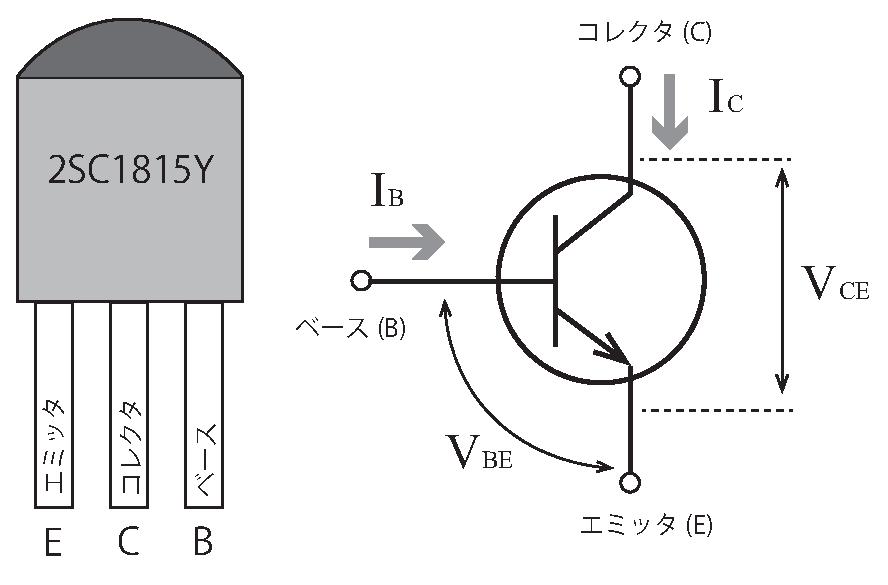
\includegraphics[keepaspectratio, scale=0.4, angle=0]
			{figs/eps/illust.eps}
			\caption{端子の名称と図記号}
			\label{fig:ex2}
		\end{figure}
	\end{multicols}
		
	\section{実習装置}
	
	\begin{multicols}{2}
		\begin{figure}[H]
			\centering
			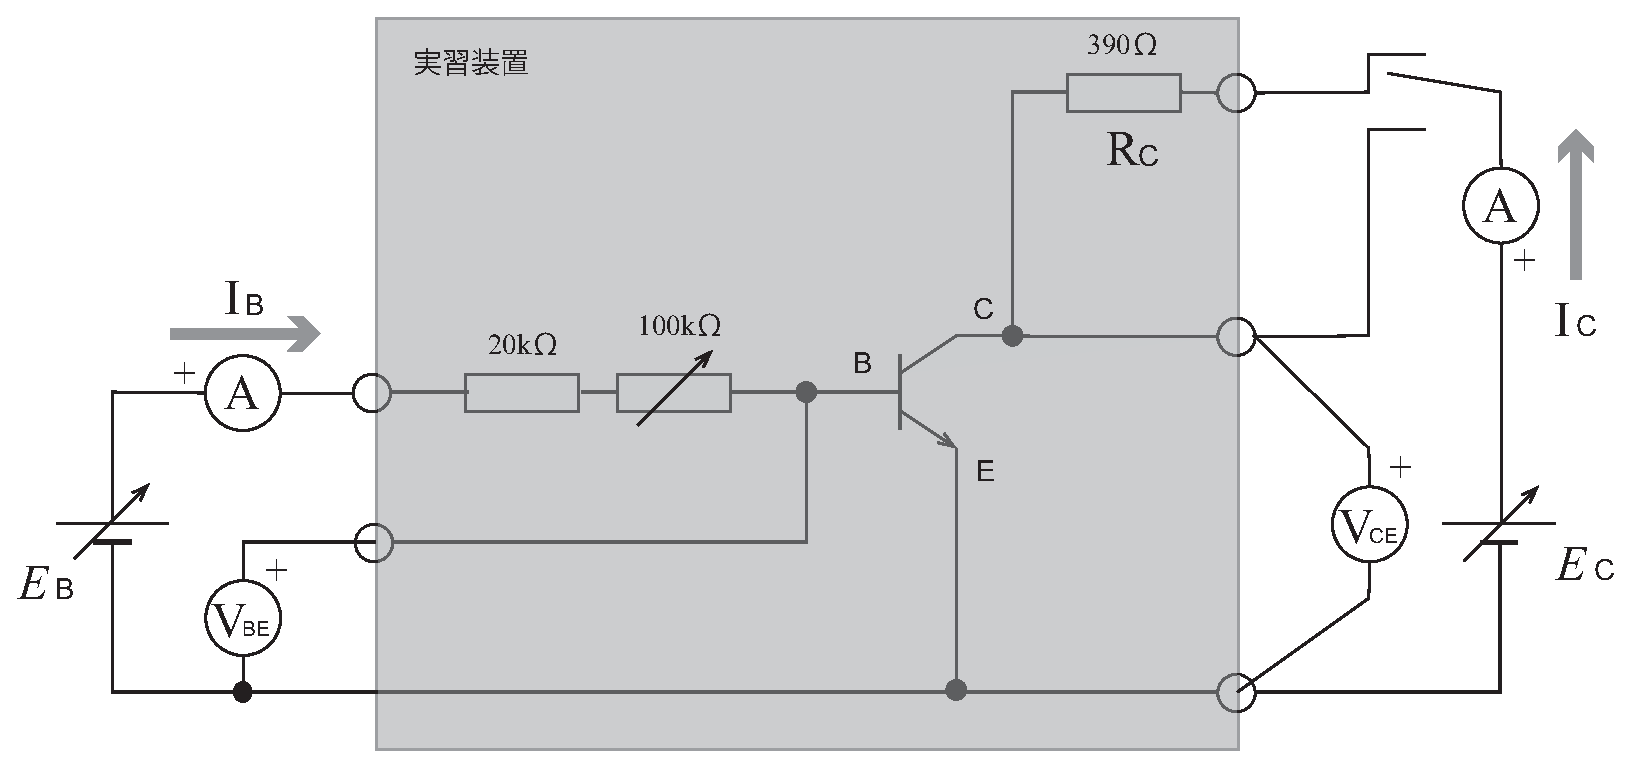
\includegraphics[keepaspectratio, scale=0.3, angle=0]
			{figs/eps/ex0.eps}
			\caption{実習回路}
			\label{fig:ex0}
		\end{figure}
		
		\begin{figure}[H]
			\centering
			\includegraphics[keepaspectratio, scale=0.161, angle=0]
			{figs/jpg/DSC_0289x.JPG}
			\caption{実習装置}
			\label{fig:ex1}
		\end{figure}
	\end{multicols}
	
	\section{結果の整理}
	
	\setlength{\voffset}{-2cm}
	\begin{figure}[H]
		\centering
		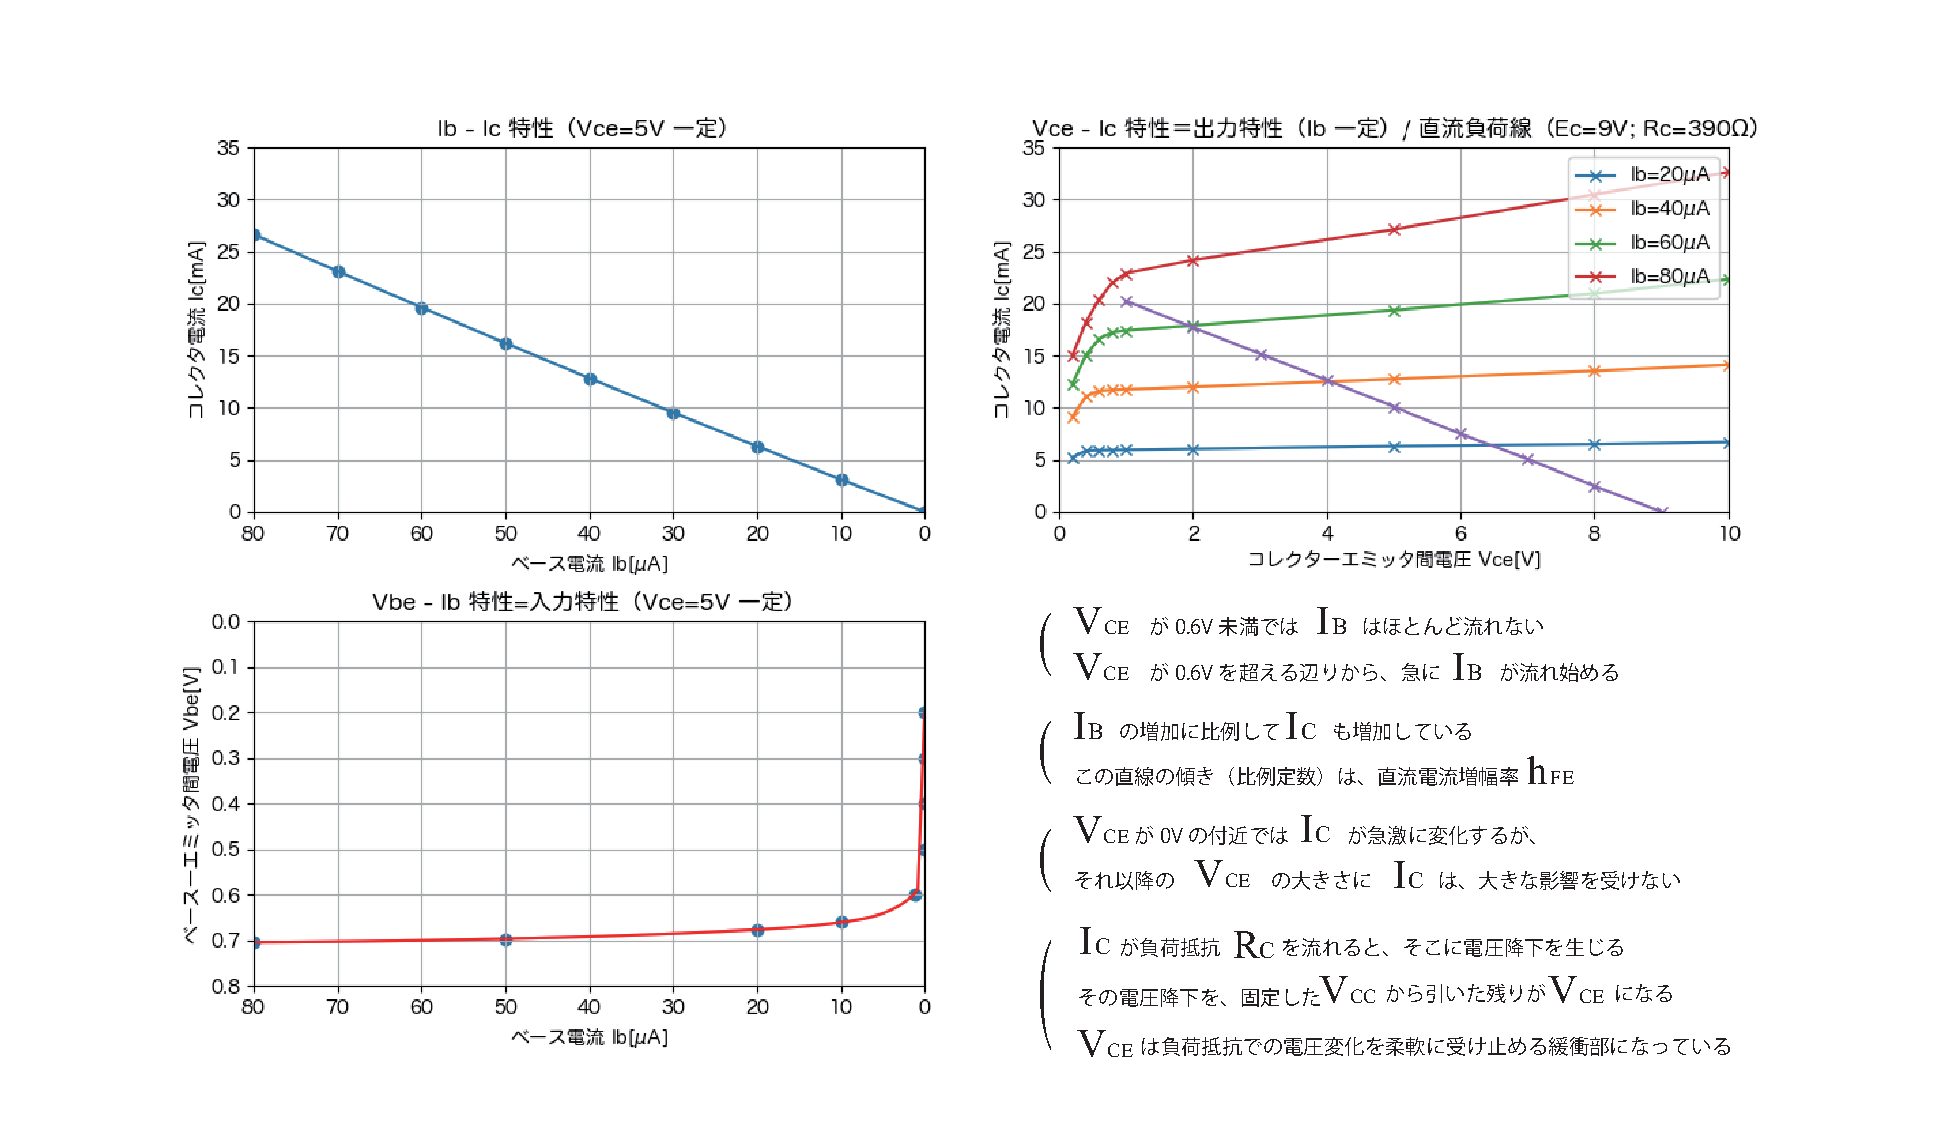
\includegraphics[keepaspectratio, scale=0.75, angle=90]
		{figs/eps/statictate.eps}
		\caption{測定結果}
		\label{fig:ex4}
	\end{figure}

\end{document}